\chapter{XSL}

\section{Conception}

Dans un premier temps, nous avions choisi de suivre une conception orientée objet, et c'est donc
naturellement que nous avons proposé une classe dédiée aux documents \textit{XSL}, proposant les
fonctionnalités de transformation d'une feuille XSL, et de même pour les instructions \textit{XSL}.

\begin{figure}[h!]
    \centering
    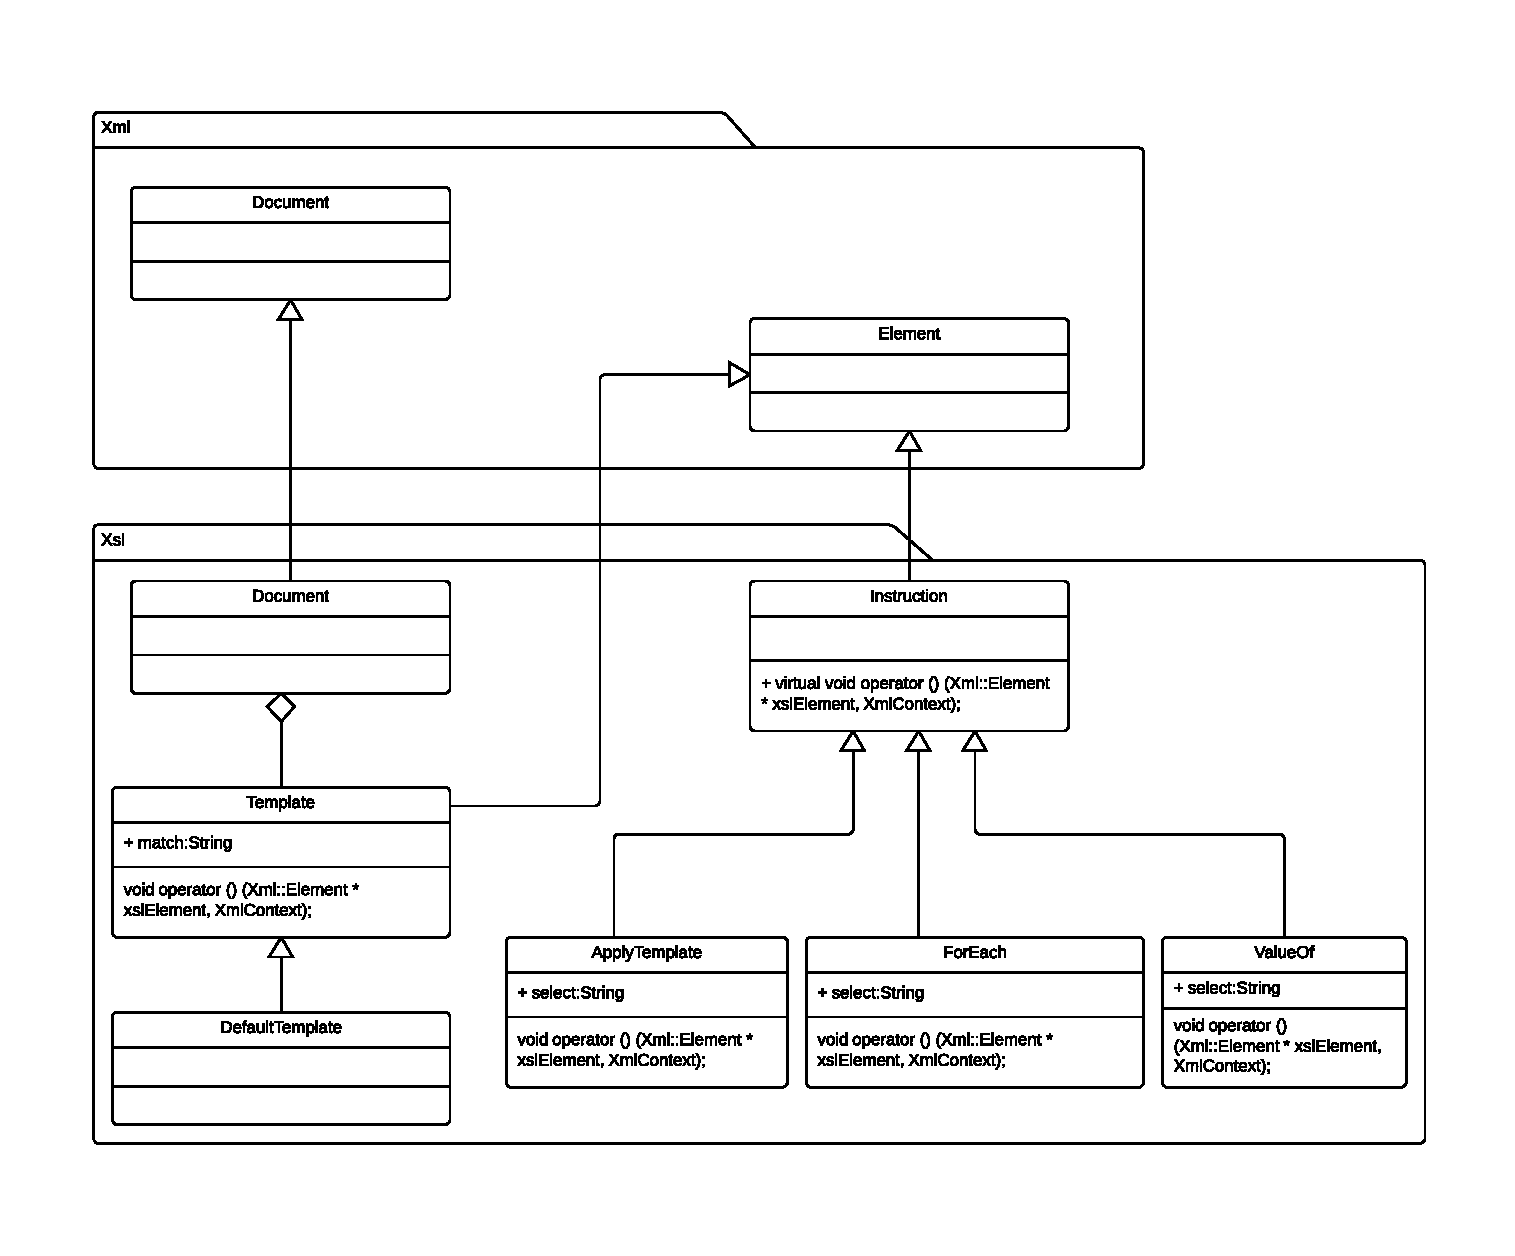
\includegraphics[width=\linewidth]{images/xsl-uml-old.pdf}
    \caption{Ancienne conception du module XSL}
    \label{oldXslClassDiagram}
\end{figure}

Néanmoins, cette conception présente de nombreux inconvénients :

En plus d'ajouter de nombreuses classe sans vraie valeur ajoutée, elle nous forçait à reconstruire l'arbre XML afin de convertir les tags
XSL en objets dédiés. On ne profitait pas réellement d'un quelconque polymorphisme non plus puisque cela demandait de toucher aux classes
XML, alors que celles ci n'ont pas comme responsabilité de gérer toutes les applications possibles de ce langage de représentation de données.

\begin{landscape}
\begin{figure}[h!]
    \centering
    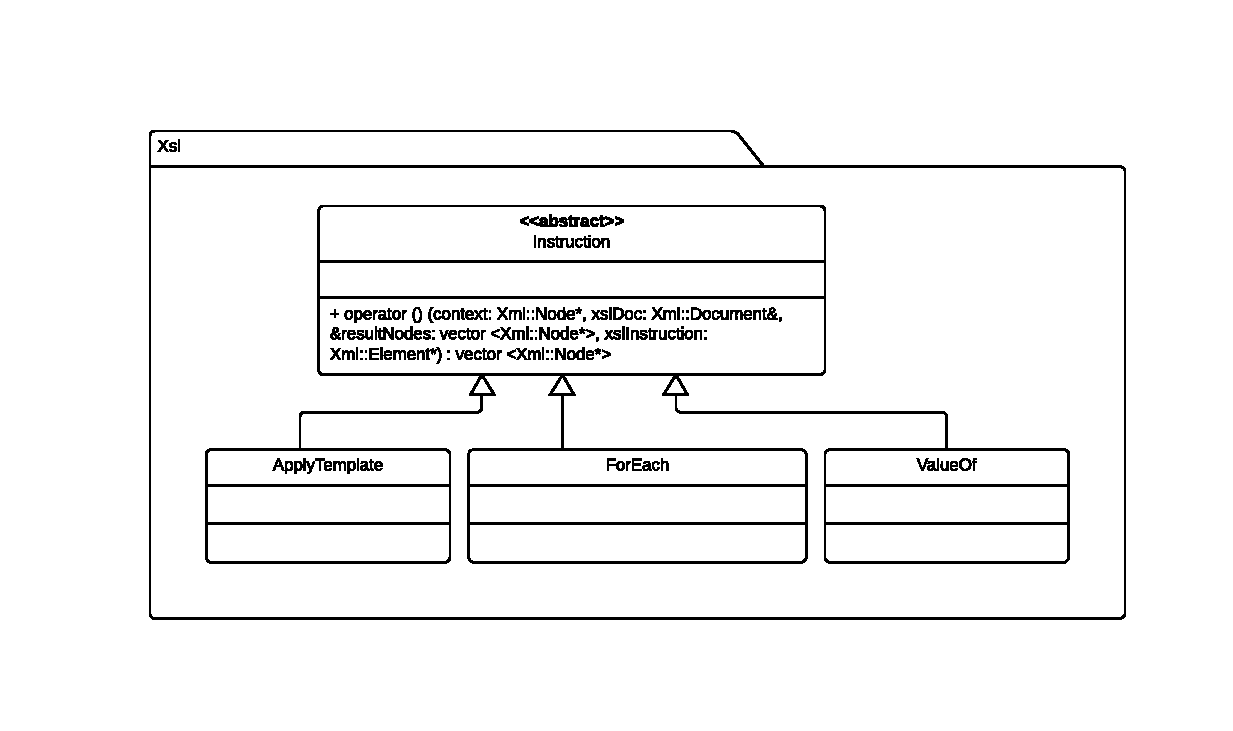
\includegraphics[width=\linewidth]{images/xsl-uml.pdf}
    \caption{Diagramme de classe des instructions XSL}
    \label{xslClassDiagram}
\end{figure}
\end{landscape}


\section{Vue globale de l'algorithme}

L'algorithme de transformation XSL s’exécute de manière récursive et bascule continuellement entre le document XSL et le document XML à transformer.

Un même algorithme s'exécute pour chaque nœud (à quelques exceptions citées ci-dessous) :

\begin{enumerate}
    \item Si le nœud n'est pas un élément, on le rajoute directement au résultat.
    \item Si un \textit{template} correspond à ce nœud, on l'applique (plus sur l'application des templates ci-dessous) en prenant ce nœud comme \textit{contexte} et on ajoute le résultat de cette application au nœud en cours de génération.
    \item Sinon, on ré-applique le même algorithme sur tous ses enfants, en ayant comme contexte l'élément actuel et en concaténant les résultats des applications de l'algorithme à tous le fils.
\end{enumerate}

La transformation XSL débute en appliquant cet algorithme à la racine du document XML à transformer, et se propage par récursions successives
à la totalité du document.

\section{Templates}

Les \textit{templates} sont les seuls fils de la racine (\textit{stylesheet}) d'un document XSL et se présentent de la manière suivante :
\\
\\
\textbf{
\lstinline$<xsl:template match="cd/title">$\\
\indent \lstinline$<tagxml></tagxml>$\\
\indent \lstinline$<xsl:uneinstruction select="untag/unautretag" />$\\
\indent \lstinline$<encoreunautretagxml />$\\
\lstinline$</xsl:template>$
}
\\
\\
Ils peuvent contenir des tags XML "normaux", ainsi que des instructions XSL.
On dit qu'un template \textit{match} un élément si l'élément est compatible avec la valeur de l'attribut \textit{match} du template, par exemple :

Si un élément XML a comme nom "title" et est le fils d'un élément qui a comme nom "cd", il match le template vu ci-dessus.

Quand on applique un template, on va renvoyer une liste de nœuds résultants (qui vont en général être ajoutés comme fils d'un document ou d'un élément). Cette liste est générée de la manière suivante :\\

\begin{enumerate}
    \item Les nœuds qui ne sont pas des éléments XML sont rajoutés directement.
    \item Les nœuds qui sont des éléments XML, mais pas XSL, sont clonés. On applique alors  puis considérés comme des templates (car pouvant contenir des instructions XSL) et appliqués avec comme contexte le nœud d'application de la transformation XSL.
    \item Les éléments XSL sont appliqués avec comme contexte le nœud d'application de la transformation XSL. Tous les nœuds résultants de cette application sont ajoutés à la liste des nœuds générés par l'application du template.
\end{enumerate}
